\chapter{Introduction}
\label{chap:intro}

Data sketches, or \emph{sketches} for short, are indispensable tools for performing analytics on high-rate, high-volume data. Specifically, understanding the data distribution is a fundamental task in data management and analysis, used in applications such as exploratory data analysis~\cite{vartak2015seedb}, operations monitoring~\cite{abraham2013scuba}, and more. 

The Quantiles sketch family captures this task~\cite{masson2019ddsketch, mergeables_summaries, gan2018moment, cormode2021relative}. The sketch represents the quantiles distribution in a stream of elements, such that for any $0 \leq \phi \leq 1$, a query for quantile $\phi$ returns an estimate of the $\lfloor n\phi \rfloor ^{\text{th}}$ largest element in a stream of size $n$. For example, quantile $\phi=0.5$ is the median. 

Due to the importance of quantiles approximation, Quantiles sketches are a part of many analytics platforms, e.g., Druid~\cite{druid-quantiles}, Hillview~\cite{budiu2019hillview}, Presto~\cite{presto}, and Spark~\cite{spark}. A case study made by Yahoo~\cite{flurry_study} has shown the impact of sketches on data analytics. Flurry~\cite{flurry} is a mobile application real-time analytics platform, acquired by Yahoo in 2014. The use of data sketches architecture in Flurry reduced the overall cost of the system considerably. Sketches led to a reduction in data processing times from days or hours to minutes or seconds.

Sketches are designed for \emph{stream} settings, in which each element is processed once. Like other sketches, Quantiles sketch is of sublinear-size and its estimates are \emph{\gls{PAC}}, providing an approximation within some error $\epsilon n$ with a failure probability bounded by some parameter $\delta$. 

The classic literature on sketches has focused on inducing a small error while using a small memory footprint, in the context of sequential processing: the sketch is built by a single thread, and queries are served only after sketch construction is complete. Only recently, we begin to see works leveraging parallel architectures to achieve a higher ingestion throughput while also enabling queries concurrently with updates~\cite{Rinberg_2020_fast_sketches, stylianopoulos2020delegation}. 
Of these, the only solution suitable for quantiles that we are aware of is the \acrfull{FCDS} framework proposed by Rinberg et al.~\cite{Rinberg_2020_fast_sketches}. However, the scalability of FCDS-based Quantiles sketches is limited unless query freshness is heavily compromised (as we show below). Our goal is to provide a scalable concurrent Quantiles sketch that retains a small error bound with reasonable query freshness.

In Chapter~\ref{chap:prelims} we formally define the system model. In Chapter~\ref{chap:background}, we define the problem and overview a popular sequential solution proposed by Agarwal et. al~\cite{mergeables_summaries} which is used by Apache DataSketches~\cite{DataSketches}, on which our concurrent sketch is based.


In Chapter~\ref{chap:quancurrent}, we present \mysketch, our highly scalable concurrent Quantiles sketch.
Like FCDS, \mysketch relies on local buffering of stream elements, which are then propagated in bulk to a shared sketch.
But \mysketch improves on FCDS by eliminating the latter's sequential propagation bottleneck, which mostly stems from the need to sort large buffers.

In \mysketch, sorting occurs at three levels – a small thread-local buffer, an intermediate \acrshort{NUMA}-node-local buffer called $\mathit{Gather\&Sort}$, and the shared sketch.
Moreover, the shared sketch itself is organized in multiple levels, which may be propagated (and sorted) concurrently by multiple threads.

To allow queries to scale as well, \mysketch serves them from a cached snapshot of the shared sketch.
This architecture is illustrated in Figure~\ref{fig:quancurrentDS}.
The query freshness depends on the sizes of local and NUMA-local buffers as well as the frequency of caching queries.
We show that using this architecture, high throughput can be achieved with much smaller buffers (hence much better freshness) than in FCDS.


% In Section~\ref{sec:background} we formally define the problem and overview a sequential solution proposed in~\cite{mergeables_summaries} and used by Apache DataSketches~\cite{DataSketches}. 
% In Section~\ref{sec:Quancurrent} we present Quancurrent, a thread-friendly version of the Quantiles sketch proposed in~\cite{mergeables_summaries}.
% We achieve high multi-threaded throughput by buffering data and propagating it to the shared sketch in bulk.
% As depicted in Figure~\ref{fig:quancurrentDS}, we use both local and shared buffers alongside a shared sketch data structure. The local buffers are non-atomically moved to the shared buffer, and the shared buffer is periodically propagated to the queryable state. The state is updated using CAS-based primitives, in a manner that ensures lock-freedom. At its base, the sequential Quantiles sketch uses a sort operation. \mysketch utilizes this mixture of local and shared buffers to mask these sorts and to allow more concurrency. 

\begin{figure}[htp]
    \centering
    % \includegraphics[width=0.8\linewidth,trim={0cm 0cm 0cm 0.3cm},clip]{graphics/algorithm/Quancurrent structure intro.pdf}
        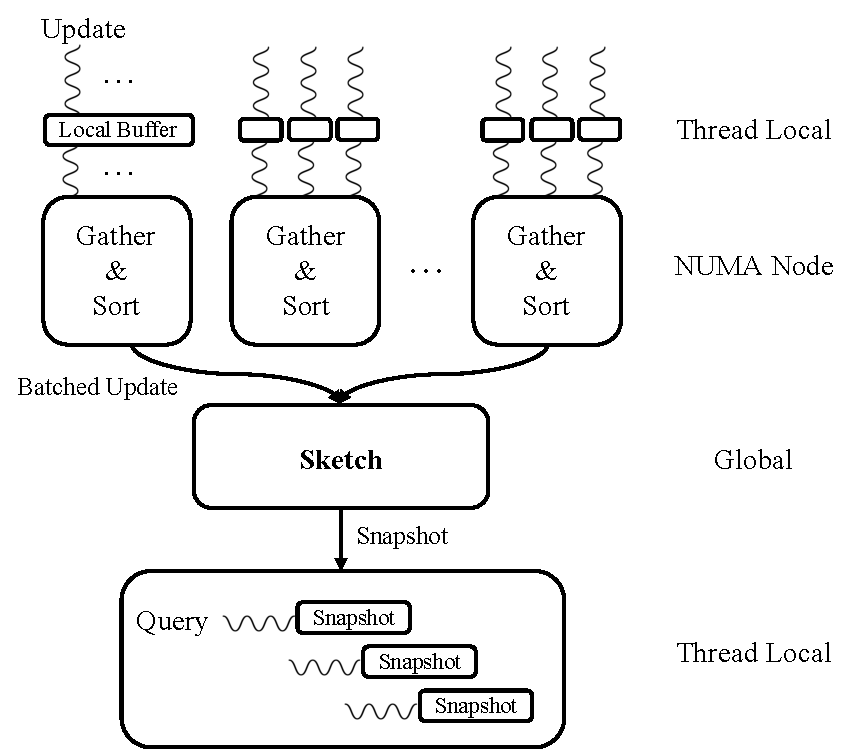
\includegraphics[width=0.8\linewidth,trim={0cm 0cm 0cm 0.3cm},clip]{graphics/algorithm/Quancurrent_structure_intro.pdf}
    \caption{\mysketch's architecture.}
    \label{fig:quancurrentDS}
\end{figure}

% For scalability purposes, queries are served from a cached snapshot of the sketch. How up-to-date the query estimation is depends on the sizes of the local and shared buffers and on the freshness of the cached snapshot, both of which are controlled by parameters.

To lower synchronization overhead, we allow buffered elements to be sporadically overwritten by others without being propagated, and others to be duplicated, i.e., propagated more than once. These occurrences, which we call \emph{holes}, alter the stream ingested by the data structure. 
Yet, in Chapter~\ref{chap:analysis} we showed that for a sufficiently large local buffer, the expected number of holes is less than $1$ and, because they are random, they do not change the sampled distribution.
Figure~\ref{fig:intro-query-accuracy} presents quantiles estimated by \mysketch on a stream of normally distributed random values compared to an exact, brute-force computation of the quantiles, and shows that the estimation remains accurate.

\begin{figure}[htp]
    \centering
    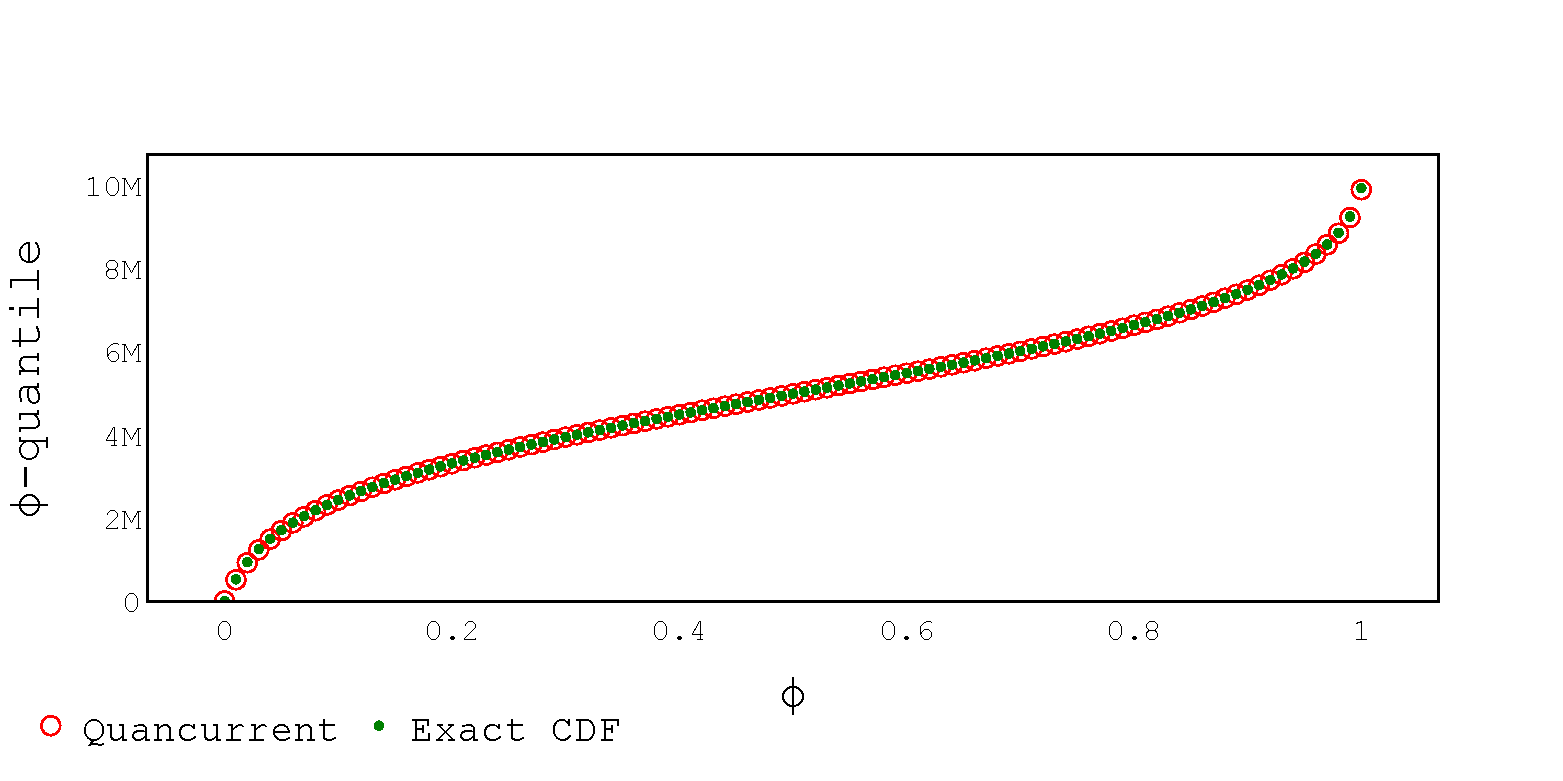
\includegraphics[width=\linewidth,trim={0cm 0.3cm 0cm 1.5cm},clip]
    {graphics/graphs/accuracy/Oracle_Quancurrent_blocking_numa_cdf_normal_k1024_b16_keys10M_runs1_uT32_qT1_snapshot1_17-09-2022_07-00-49.pdf}
    \caption{\mysketch quantiles vs. exact CDF, k = 1024, normal distribution, 32 update threads, 10M elements.}
    \label{fig:intro-query-accuracy}
\end{figure}


In Chapter~\ref{chap:eval} we empirically evaluate \mysketch. We show an update speedup of $12$x and a query speedup of $30$x over the sequential sketch, both with linear speedup. We compare \mysketch to FCDS, which is the state-of-the-art in concurrent sketches, and show that for FCDS to achieve similar performance it requires an order of magnitude larger buffers that \mysketch, reducing query freshness tenfold.

In Chapter~\ref{chap:correctness} we present a formal correctness proof. 


